\section{Overview of \lm}

\begin{figure*}
    \centering
    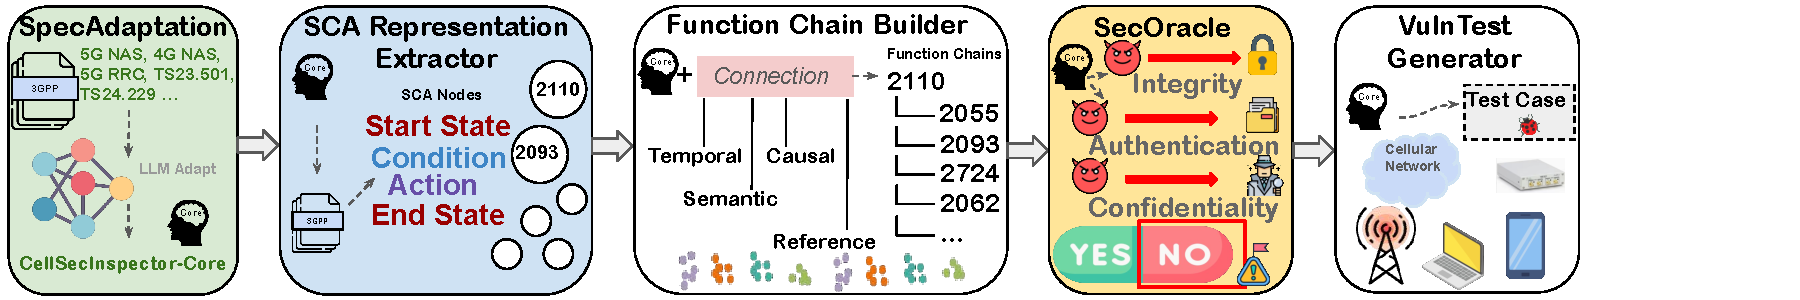
\includegraphics[width=0.82\linewidth]{pic/Overview.pdf}
    \vspace{-0.1in}
    \caption{\lm Overview}
    \label{fig:Overview}

\end{figure*}

\subsection{Approach Skeleton}
Figure~\ref{fig:Overview} shows the overview of \lm, which can automatically comprehend complicated 3GPP specifications, model the mobile network functions using structured state-condition-action (SCA) representations, and examine whether the 3GPP-designed procedures can violate foundational security properties. Five primary modules of \lm are developed: \textit{SpecAdaptation} (\ul{Spec}ification \ul{Adaptation}), \textit{SCA Representation Extractor}, \textit{Function Chain Builder}, \textit{SecOracle} (\ul{Sec}urity \ul{Oracle}), and \textit{VulnTestGenerator} (\ul{Vuln}erability \ul{Test} \ul{Generator}). 
\textit{SpecAdaptation} adapts the core model \textit{CellSec\-Inspector-Core} to the cellular network domain knowledge using the collected and curated 3GPP specifications. \textit{CellSecInspector\allowbreak-Core} is further used in later modules.
Two components are involved to comprehensively model the complicated mobile network functions. \textit{SCA Representation Extractor} parses and extracts the SCA nodes from 3GPP specifications and the internal domain knowledge learned via \textit{SpecAdaptation}. \textit{Function Chain Builder} connects scattered SCA nodes into function chains for comprehensively modeling the cellular network services specified in 3GPP specifications. Next, \textit{SecOracle} conducts the security checking using the foundational security properties. Lastly, \textit{VulnTestGenerator} automatically generates test cases for candidate violations. 


\subsection{Challenges and Insights}
\label{subsect:challenges}

3GPP specifications are inherently complex and have a vast scope, complicating the development of a framework for comprehending the cellular networks governed by 3GPP specifications. For instance, NAS and RRC specifications span thousands of pages, with intricate interdependencies and frequent updates across releases. A single 5G NAS specification TS 24.501 contains over \texttt{981} pages~\cite{3GPP_TS_24501}. Reading and understanding 3GPP specifications is a time-consuming challenge even for experts. We design and develop \lm based on a pretrained LLM. 
To enable \lm to discover vulnerabilities from 3GPP specifications, we solve three main challenges.  

\noindent \textbf{C1: Lack of annotated resources for mobile network security research tasks.}
Different from common NLP (natural language processing) research tasks, such as text classification, that come with the thorough and well-annotated datasets, there are no well-known and easily accessible resources in the mobile network research community. Specifically, we need to model the complex mobile network procedures first to conduct the security analysis of mobile network functions and services. Unfortunately, there are no established and public annotation specifications or training resources in this domain-specific task. 

\noindent $\diamond$ \textbf{Insight1:} To address C1, we propose the \textit{SCA Representation Extractor}, which is designed to extract information for modeling the mobile network functions and services from 3GPP specifications. Two approaches are developed. First, instead of constructing the traditional FSM (finite state machine) models, \textit{SCA Representation Extractor} captures the self-contained transition of mobile network procedures in our proposed \textit{SCA (State-Condition-Action)} structure that can compose the complex and completed function event in a single presentation. Second, we adopt the efficient few-shot In-Context Learning (ICL) to enable our system to extract SCA nodes without large-scale annotated datasets. 

\noindent {\textbf{C2: Computational cost for linking SCA nodes at scale.} 
After deriving scattered SCA nodes, these nodes must be linked to construct complete mobile network procedures and capture the comprehensive network status (e.g., whether the security context is established). 

However, linking SCA nodes at scale is challenging because different procedures described in SCA nodes may or may not share meaningful relationships. 
Moreover, to avoid redundancy, 3GPP specifications use cross-references between clauses and specifications, further complicating the linkage process.  
With thousands or more SCA nodes that can create millions of candidate connections in a quadratic manner, it imposes substantial computational overhead for linking SCA nodes at scale. 

\noindent $\diamond$ \textbf{Insight2:} 
To address C2, we introduce the \textit{Function Chain Builder}, which integrates two approaches: Type I: Node-Informed Exhaustive Connection and Type II: Reference Guided Connection.
Type I compares all node pairs to identify three types of valid transitions: temporal connections that link nodes with identical end and start states, semantic connections that capture equivalent but textually different states, and causal connections where one node’s state, condition, or action enables another. While Type I provides comprehensive coverage, its $O(n^2)$ complexity is costly as the number of nodes grows. To reduce this burden, Type II leverages the rich cross-references embedded in 3GPP specifications (e.g., `\textit{as specified in subclause X.Y.Z}') to restrict the search space to relevant sections. Together, these strategies enable efficient and automated construction of function chains across 3GPP specifications.

\noindent \textbf{C3: Manually crafted security requirements are impractical for security assessment of large-scale mobile network functions.} 
State-of-the-art methods, such as \textit{Hermes}~\cite{al2024hermes}  and \textit{ConTester}~\cite{chen2023sherlock}, rely on a small set of manually crafted security  requir-\ ements for specific procedures. For example, ConTester’s security requirement S6 mandates that `\textit{Except the messages listed below, no NAS signaling messages shall be processed by the receiving EMM entity in the UE forwarded to the ESM entity, ...}', which is the sentence directly from TS 24.301 subclause 4.4.4.2. When new NAS procedures are introduced in subsequent 3GPP releases, if these sentences are updated, their security requirements must be manually revised, limiting the scalability for the security assessments of large-scale mobile network functions. Similarly, approaches that build FSM models also need to manually translate FSM models into SMV language~\cite{clarke1996symbolic,al2024hermes,hussain20195greasoner,hussain2018lteinspector} to enable formal security analysis, requiring significant expert efforts that are not practical given the complexity and breadth of modern mobile networks.  

\noindent $\diamond$ \textbf{Insight3:} We develop the \textit{SecOracle} that introduces 9 foundational security properties. 
\textit{Unlike procedure-specific requirements, these properties are derived from classic and foundational security principles applicable across the entire mobile network stack. }
Therefore, \textit{SecOracle} can operate on large-scale cellular network procedures with broader security checkpoints. This equips \lm with the foundational ability to detect previously unreported vulnerabilities.